\captionsetup[subfigure]{labelformat=empty}

\begin{tikzpicture}[zoomboxarray, zoomboxes below, zoomboxarray inner gap=0.4cm,
zoomboxarray columns=4, zoomboxarray rows=2,remember picture, black and white]
   \node [image node] {
   \setcounter{zoombox}{0} 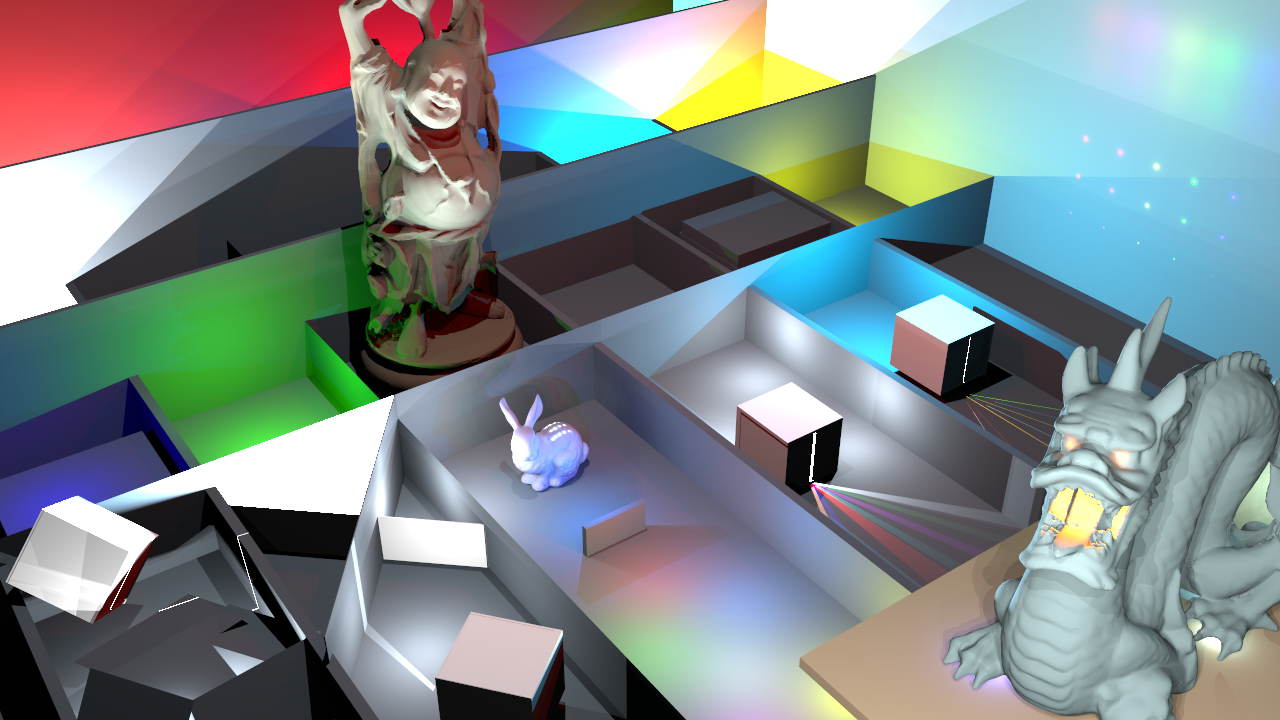
\includegraphics[width=1\textwidth]{figures/StanfordMuseum_ref.png}};
   
   \zoombox[magnification=0.8, color code=red]{0.85,0.3}
   \zoombox[magnification=1.5, color code=yellow]{0.334,0.78}
   
   \zoombox[magnification=2.3, color code=green]{0.767,0.47}
   \zoombox[magnification=1.4, color code=olive]{0.895,0.79}
   
   \zoombox[magnification=2, color code=brown]{0.285,0.32}
   \zoombox[magnification=1.3, color code=blue]{0.11,0.2}
   
   \zoombox[magnification=1.5, color code=cyan]{0.12,0.72}
   \zoombox[magnification=2, color code=pink]{0.6,0.68}

\end{tikzpicture}
\begin{tikzpicture}[overlay,remember picture]

\foreach \X in {1,...,\thezoombox}
   {\node[anchor=south,yshift=-13pt] at (zoombox-\X.south) 
   {\tiny (\X)};}
   \setcounter{zoombox}{0} 
\end{tikzpicture}
